
        % Define grid dimensions
\documentclass{article}
\usepackage{tikz}
\usepackage{caption}
\usepackage{adjustbox}
\newcommand{\pyvar}[1]{\texttt{#1}}
\begin{document}


\begin{figure}[h]
    \centering
        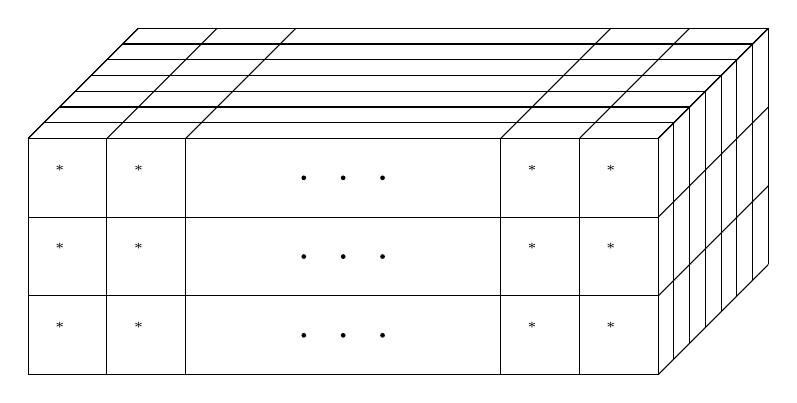
\begin{tikzpicture}
    
    
    % Define grid dimensions
    
    
    \def\n{3} % N = 1 row (front face height)
    \def\m{8} % M = 20 columns (front face width)
    \def\l{3} % M = 20 columns (front face width)
    \def\r{5} % M = 20 columns (front face width)
    \def\depth{7} % Depth of the cube (z-axis, number of cells in depth)
    \def\cellsize{1} % Size of each cell
    \def\xoffset{24.5}
    \def\yoffset{2}

    % Define 3D perspective skew for top and right faces
    \def\skewx{0.2} % Skew factor for x-axis (right face)
    \def\skewy{0.2} % Skew factor for y-axis (top face)

    % --- Front Face (the original 1x20 grid) ---
    % Draw the grid - Horizontal lines
    \foreach \i in {0,...,\n} {
        \draw[black] (-\xoffset,\i*\cellsize+\yoffset) -- (-\xoffset+\m*\cellsize,\i*\cellsize+\yoffset); % Horizontal lines
    }

    % Draw the grid - Vertical lines with condition
    \foreach \j in {0,...,\m} {
        \ifnum\j<\l % Check if j < 7
            \draw[black] ((-\xoffset+\j*\cellsize,+\yoffset) -- ((-\xoffset+\j*\cellsize,\n*\cellsize+\yoffset); % Draw line
        \else
            \ifnum\j>\r% Check if j > 13
                \draw[black] ((-\xoffset+\j*\cellsize,\yoffset) -- ((-\xoffset+\j*\cellsize,\n*\cellsize+\yoffset); % Draw line
            \fi
        \fi
    }

    % % Place dots in the middle of the front face (simulating row 3 in a 5-row grid, but here it's the only row)
    % \foreach \j in {0,1,2} {
    %     \fill[black] ({(1-\j)/2+\m*\cellsize/2}, 0.5*\cellsize) circle (0.03); % Dots
    % }

% Assuming \cellsize and \m are defined, and \n is the number of rows
\foreach \i in {0,...,\numexpr\n-1} { % Loop over rows
    \foreach \j in {0,1,2} { % Three dots per row
        \fill[black] ({(-\xoffset+(1-\j)/2+\m*\cellsize/2}, {((\n-1-\i)*\cellsize+0.5*\cellsize+\yoffset}) circle (0.03); % Dots
    }
}
    % Draw the outer rectangle for the front face
    \draw[black] ((-\xoffset,\yoffset) rectangle (-\xoffset+\m*\cellsize, \n*\cellsize+\yoffset);

    % Add the shape label below the grid

    % Assuming \cellsize and \n are defined
\foreach \i in {0,...,\numexpr\n-1} { % Loop over rows
    \node at ((-\xoffset+0.4*\cellsize, {(\n-1-\i)*\cellsize+0.6*\cellsize+\yoffset}) {\tiny *};
    \node at (-\xoffset+1.4*\cellsize, {(\n-1-\i)*\cellsize+0.6*\cellsize+\yoffset}) {\tiny *};
    \node at (-\xoffset+6.4*\cellsize, {(\n-1-\i)*\cellsize+0.6*\cellsize+\yoffset}) {\tiny *};
    \node at (-\xoffset+7.4*\cellsize, {(\n-1-\i)*\cellsize+0.6*\cellsize+\yoffset}) {\tiny *};
}

    % \node at (0.4*\cellsize, \n*\cellsize-0.4*\cellsize) {\tiny *};
    % \node at (1.4*\cellsize, \n*\cellsize-0.4*\cellsize) {\tiny *};
    % \node at (6.4*\cellsize, \n*\cellsize-0.4*\cellsize) {\tiny *};
    % \node at (7.4*\cellsize, \n*\cellsize-0.4*\cellsize) {\tiny *};


    % --- Top Face ---
    % Draw the top face as a parallelogram
    \draw[black] (-\xoffset+\m*\cellsize, \n*\cellsize+\yoffset) -- ++(\depth*\cellsize*\skewx, \depth*\cellsize*\skewy); % Right edge of top face
    \draw[black] ((-\xoffset, \n*\cellsize+\yoffset) -- ++(\depth*\cellsize*\skewx, \depth*\cellsize*\skewy); % Left edge of top face
    \draw[black] ((-\xoffset+\m*\cellsize, \n*\cellsize+\yoffset) -- ((-\xoffset, \n*\cellsize+\yoffset); % Front edge (already drawn)
    \draw[black] ((-\xoffset+\m*\cellsize+\depth*\cellsize*\skewx, \yoffset+\n*\cellsize+\depth*\cellsize*\skewy) -- (-\xoffset+\depth*\cellsize*\skewx, +\yoffset+\n*\cellsize+\depth*\cellsize*\skewy); % Back edge

    % Draw grid lines on the top face (along x-axis)
    \foreach \j in {0,...,\m} {
        \ifnum\j<\l % Same condition as front face
            \draw[black] (-\xoffset+\j*\cellsize, \n*\cellsize+\yoffset) -- ++(\depth*\cellsize*\skewx, \depth*\cellsize*\skewy);
        \else
            \ifnum\j>\r
                \draw[black] (-\xoffset+\j*\cellsize, \n*\cellsize+\yoffset) -- ++(\depth*\cellsize*\skewx, \depth*\cellsize*\skewy);
            \fi
        \fi
    }

    % Draw grid lines on the top face (along z-axis, depth)
    \foreach \k in {0,...,\depth} {
        \draw[black] (-\xoffset+\m*\cellsize+\k*\cellsize*\skewx, \yoffset+\n*\cellsize+\k*\cellsize*\skewy) -- (-\xoffset+\k*\cellsize*\skewx, \yoffset+\n*\cellsize+\k*\cellsize*\skewy);
    }

    % --- Right Face ---
    % Draw the right face as a parallelogram
    % \draw[lightgray] (\m*\cellsize, \n*\cellsize) -- ++(\depth*\cellsize*\skewx, -\depth*\cellsize*\skewy); % Top edge of right face
    % \draw[lightgray] (\m*\cellsize, 0) -- ++(\depth*\cellsize*\skewx, -\depth*\cellsize*\skewy); % Bottom edge of right face
    \draw[black] (-\xoffset+\m*\cellsize, \yoffset+\n*\cellsize) -- (-\xoffset+\m*\cellsize, \yoffset); % Front edge (already drawn)
    % \draw[lightgray] (\m*\cellsize+\depth*\cellsize*\skewx, \n*\cellsize-\depth*\cellsize*\skewy) -- (\m*\cellsize+\depth*\cellsize*\skewx, -\depth*\cellsize*\skewy); % Back edge

    % Draw grid lines on the right face (along y-axis, height)
    \foreach \i in {0,...,\n} {
        \draw[black] (-\xoffset+\m*\cellsize, \yoffset+\i*\cellsize) -- ++(\depth*\cellsize*\skewx, \depth*\cellsize*\skewy);
    }

\foreach \k in {0,...,\depth} {
    \draw[black] (-\xoffset+\m*\cellsize+\k*\cellsize*\skewx, \yoffset+\n*\cellsize+\k*\cellsize*\skewy) -- (-\xoffset+\m*\cellsize+\k*\cellsize*\skewx, \yoffset+\k*\cellsize*\skewy);
}

    \end{tikzpicture}
\end{figure}
\end{document}